\chapter{Flow Monitoring Performance}\label{chap:flow-monitoring-performance}

% TODO user-space -> use space, same with kernel, zvazit pomlcku u pridavnych jmen

\begin{chapintro}

Monitoring of high-speed networks is becoming a resource-intensive task. There are dedicated flow monitoring probes built with commodity hardware support up to 10\,G links, but multiple 10\,G or even 100\,G optical networks are being used for transport networks and a data centre connectivity. Moreover, application flow monitoring is even more demanding than the basic flow monitoring. Therefore, the performance of flow monitoring is an important topic.

The goal of this chapter is to describe how the performance of flow monitoring can be measured and what steps can be taken to improve the performance. We describe the state-of-the-art in packet capture, which is an essential part of every flow monitoring system. We show which parts of the packet capture directly influence the design of the flow monitoring process and discuss how the flow monitoring can take advantage of the different features provided by packet capture frameworks. Description of the most impactful optimization techniques both with and without the use of specialized FPGA-based network interface cards is provided. Moreover, several novel techniques for improving flow monitoring performance are proposed as well.

Running and maintaining many separate probes is uneconomical and time-consuming. Therefore, we explore the possibility to facilitate network interface cards (NICs) with multiple 10\,G interfaces to build probes which can replace many existing boxes, leading to reduced management and operational costs. The monitoring performance is critical for such a high-density solution. We use two custom-built, FPGA-based NICs, each with eight 10\,G interfaces to test current CPU limits and to propose improvements for the near future commodity NICs.

The paper included in this chapter is~\cite{Velan-2015-High}. %Another
Paper related to this chapter is~\cite{Pus-2015-Hardware}.

The organisation of this chapter is as follows:
\begin{itemize}
  \item Section~\ref{sec:performance-measurement} provides background to the measurement of flow monitoring performance and highlight its pitfalls.
  \item Section~\ref{sec:performance-capture} describes the state-of-the-art of high-speed packet capture, which is an important part of every flow monitoring system.
  \item Section~\ref{sec:performance-hw-acceleration} shows how can the flow monitoring be accelerated with the use of specialized FPGA-based network interface cards.
  \item Section~\ref{sec:performance-sw-optimization} discusses available methods of optimization of flow exporter software.
  \item Section~\ref{sec:performance-high-density} presents a high-density flow monitoring system capable of monitoring of sixteen 10\,Gb links in a single box and evaluates its performance.
  \item Section~\ref{sec:performance-summary} summarizes the chapter.
\end{itemize}

\end{chapintro}

\newpage


\section{Measuring Flow Monitoring Performance}\label{sec:performance-measurement}

The primary goal of measuring flow monitoring performance is to determine whether the system can be deployed to monitor a particular network or a link. For example, if the system is capable of monitoring 20\,Gb/s of traffic, it can be deployed in both directions of a 10\,Gb/s link. However, the claim that the system can handle 20\,Gb/s may mean a lot of different things and it usually differs from vendor to vendor. The throughput of a flow monitoring process depends on a number of factors, such as the configuration of the flow creation process and the type of network traffic that is being monitored. 10\,Gb/s may mean 14.88\,Mpps (millions of packets per second) for minimum Ethernet frames (20\,B + 64\,B) or just 813\,kpps for maximum Ethernet frames on 1500\,MTU (each frame is 1538\,B). The processing of different packet headers can take different time as well, for example, IPv4 vs IPv6 or UDP vs TCP. The number of flows has a large impact on the flow creation process as a flow record must be kept for each of the flows. Therefore, a detailed performance analysis of the flow monitoring system should be performed before its real-world deployment.

The throughput of the flow monitoring system is usually measured either in packets per second or bits per second. However, since the packet size should be reported as well so that these values provide meaningful information, they are mostly interchangeable. Packets per second metric is preferred in most of this chapter.

The goal of this section is two-fold. Firstly, it describes the parameters that need to be specified when reporting on a flow monitoring system performance. There are three different categories of the parameters: hardware configuration, exporter configuration, traffic composition. Secondly, measurement of the impact of optimizations is discussed. Although the impact can be measured simply by an increase in the overall throughput, there are a few pitfalls that need to be recognized and avoided for the results to be interpreted correctly.


\subsection{Measuring Overall Throughput}

The overall throughput of the flow monitoring process depends upon a number of factors. Moreover, there are two methods of measuring the throughput even if all of these factors are set. The first method is to generate the testing traffic at such a rate that is above the capability of the monitoring process to handle. The throughput is then determined as the number of packets that were actually processed by the flow exporter. This method gives an upper bound on the capabilities of the monitoring process and the measurement is quite easy to carry out. However, deploying the flow monitoring system based on such an estimate can easily lead to dropped packets in practice since there is quite a large packet drop associated with the measurement as well. The second method measures throughput without packet loss or with a defined packet loss rate. Given a predetermined packet loss rate, the traffic is generated so that the flow monitoring system performs with lower that given packet loss rate. The throughput is then increased until the packet loss matches the predetermined value and the throughput at that point is considered to be the result of the measurement. Both performance measurement methods are important. The first one gives an upper bound of the capabilities of the flow monitoring process and the second one shows how much traffic can be safely processed with acceptable packet loss.

When evaluating the performance of a flow monitoring process, the hardware on which it runs must be taken into consideration. The performance depends on the frequency of the processor, available instruction sets, and size of caches. When the exporter software is able to utilize multiple threads the number of cores of the processor and the number of processors matter as well. Moreover, when there is more than one processor, the correct use of Non-Uniform Memory Access (NUMA) architecture is important. The buffers of processes and threads running on a one CPU should be in a memory connected to the same CPU. Otherwise, the latency for accessing this memory is increased as the data must be accessed by a memory controller of another process through a bus such, as the QuickPath Interconnect~\cite{IntelCorporation-2009-Introduction} bus or its newer version Ultra Path Interconnect (in case of Intel processors).

The choice of packet capture solution often limits the upper bound on the throughput of the flow monitoring process. Although packet capture is an important part of flow monitoring process, it is used for other tasks as well and is of interest to various researchers~\cite{Garcia-Dorado-2013-High, Nassopulos-2014-Flow}. High-speed packet capture is described in more detail in Section~\ref{sec:performance-capture}.

The configuration of the flow exporter has a great impact on the throughput as well. The active and inactive timeouts significantly affect the number of created flows and flow records~\cite{Hofstede-2014-Flow} which in turn affects the utilization of the flow cache and therefore the total throughput. The flow cache size should be tuned to the expected number of flows so that the data locality is preserved as much as possible. Moreover, the size of flow records depends on the number of extracted properties and it affects the size of the cache as well. The more properties extracted, the larger the flow record. Naturally, the number of extracted properties has a direct impact on the throughput since each property must be extracted and stored in the flow record, which requires computing power and more memory accesses.

One of the most important aspects of throughput measurement is the used dataset. Choosing shortest packets and a single flow allows to benchmark the packet parser, shortest packets and a large number of flows put great stress on the flow cache. Using more complex packets with multiple protocol layers tests the packet parser capabilities and performance as well. The relative sizes of flows in the dataset matter as well. When there are a few dominant flows, the corresponding flow records are kept cached and the overall performance increases. However, if the packets of the flows are equally interlaced, the caching of the flow records is limited. Since the choice of the dataset has such an extensive impact on the flow monitoring process and its throughput, it is imperative to choose a correct dataset that supports the intentions of the given benchmark. A guidance for choosing a dataset can be found in the work of the IETF Internet IP Performance Measurement working group~\cite{IESG-1997-IP} and IETF Benchmarking Methodology working group~\cite{IESG-1989-Benchmarking}, especially in~\cite{rfc2330, rfc6985}.

We have argued that there are many factors that influence the throughput of a flow monitoring system. Since it is clearly not possible to test all combinations of the input parameters, it is necessary to choose a set of appropriate settings that cover either the most extreme scenarios or approximate some important real-world scenario. The work of~\citeauthor{Nassopulos-2014-Flow}~\cite{Nassopulos-2014-Flow} shows that performing a measurement using a large number of configurations allows deriving results that can help with the optimization effort. They show that the implementation of the flow cache as well as the composition of the traffic has a large impact on the flow monitoring process. Regardless of the chosen parameters, a proper description of the used configuration and dataset must always accompany all presented results. Therefore, we recommend using a synthetic dataset that can be described in a few simple rules.


\subsection{Measuring an Impact of Optimizations}

Throughput measurement is an integral part of any performance optimization effort. The goal of the measurement, in this case, is two-fold. Firstly, bottlenecks and need to be identified so that the optimization can be effective. For example, if a flow cache lookup takes 70\,\% of the total processing time for a single packet, optimizing packet parser is not very effective. Secondly, the measurement is repeated to examine the effect of a given optimization. Moreover, it is necessary to verify that optimizing for a single use case does not have a negative impact on other use cases. Therefore, a thorough performance measurement is repeated often during any optimization process.

Identifying bottlenecks can be a complicated process. It is often beneficial to measure execution time spent on processing a single packet throughout the flow monitoring process. The authors of~\cite{NETCOPETechnologies-2017-Modelling} show that it is possible to roughly estimate the time required for packet reception and parsing based on several parameters. \citeauthor{Gallenmueller-2015-Comparison} apply a similar methodology to compare the performance of several high-performance packet processing frameworks in~\cite{Gallenmueller-2015-Comparison}. Using a similar process can help to identify bottlenecks in the flow processing as well.

The processing speed of a computer is limited by the speed of the processor and the time required to fetch data from memory. If a computation requires only a small amount of memory that fits in CPU registers or L1 cache, the processor can be fully utilized. However, when a lot of data needs to be processed, there are many uncached accessed to memory with high latency. This causes the CPU utilization to be low. Moreover, the memory bus utilization is higher since the data needs to be transferred from RAM to CPU cache more often. Therefore, it is very useful to measure the number of instructions per processor cycle (IPC). The higher the IPC, the better the CPU is utilized. When optimizing such a process, the computation should be simplified. However, when the IPC is low, the CPU waits for data from memory. In such a case, optimizing data locality and memory accesses is the best way to improve the performance. 

Since multi-core CPUs are a standard nowadays, a good way to improve performance is to process the data using multiple threads. However, it is important to keep in mind that the bandwidth of CPU memory controller is limited and that passing data between the threads consumes the bandwidth as well. Finding a good balance is often a difficult task which requires experimentation and thorough measurement of the system load.

A good way to understand the relationship between CPU processing power and memory bandwidth is to use Roofline Performance Model~\cite{Williams-2009-Roofline}. Its core parameter is Arithmetic Intensity which is the ratio of total floating-point operations to total data movement. The visualisation of the model shows both the implementation performance limitation and limitations of the used architecture. However, correctly estimating the arithmetic intensity of the flow measurement process is a challenging task.

Optimizations proposed in Sections~\ref{sec:performance-hw-acceleration} and~\ref{sec:performance-sw-optimization} either reduce the amount of processed data or reduce the number of computation steps necessary to process each packet. We also discuss multithreaded flow processing and point out the pitfalls and caveats that can result in incorrect results.


\section{High-Speed Packet Capture}\label{sec:performance-capture}

Packet capture is the first step of the flow monitoring process and has a significant impact on the overall performance. Moreover, as it is an important part of other network applications, such as switching and routing~\cite{Kawashima-2016-Host}, the high-speed packet capture using commodity hardware running Linux operating system has been an active research area in recent years. Since the performance of packet capture directly impacts the performance of the whole flow monitoring process, the aim of this section is to present basic principles and significant technologies in this area. Furthermore, some techniques of the packet capture, such as Receive Side Scaling (RSS), have a direct impact on the functionality of flow monitoring as well.

The goal of high-speed packet capture is to deliver packets from Network Interface Card (NIC) to the user-space application as fast as possible while providing the desired functionality, such as packet fanout to multiple threads and applications. The main difference between high-speed packet capture and standard packet processing in an operating system is that the high-speed packet capture is not connection oriented. It does not provide socket API for applications to easily communicate through. Instead, it allows applications to effectively receive and send raw packets. However, to understand the packet capture process and its limitations, we shortly describe how Linux network stack receives packets, as it is the common starting point of all packet capture frameworks.

\subsection{Linux Network Stack}

The basic function of every NIC is to receive a packet from the network and pass it to the RAM memory, where it is processed further. Direct Memory Access (DMA) is used for the data transfer. The main advantage is that it does not require the cooperation of the CPU and does not consume any CPU cycles. The NIC can access only a limited memory region for which the DMA access is permitted. In the Linux network stack, this region is part of the kernel memory and is not directly accessible to the user-space. The way to notify the kernel of arrival used to be through Interrupt ReQuest (IRQ). However, as the network speed increased to 1\,Gbps speed, full utilization of the network used to cause an interrupt storm -- way too many interrupts for the system to handle efficiently. The original network stack was replaced by New API (usually called NAPI), which uses polling for high-speed packet reception and falls back to interrupts for lower packet rates. This combination of both interrupt and polling approaches allows to consume CPU cycles for low traffic and avoids interrupt storms for high packet rates. The NAPI was introduced in Linux kernel version 2.4.20 and 2.6.

After the packet is present in RAM and the kernel is notified, either by interrupt or polling, the packet is copied to kernel internal structure called \emph{sk\_buff}. Modern NIC drivers support copying of packets directly to a \emph{sk\_buff} structure, which eliminates the copying and increases performance. The \emph{sk\_buff} structure is then pushed to kernel network stack, where it is processed and made available to user applications. However, every call to a system \emph{recv*} function also needs to provide a pointer to an user-space buffer to which the data are copied. Therefore, the packet is copied at least once by the kernel, as demonstrated in Figure~\ref{fig:NAPI_no_MMAP}. Moreover, before the \emph{recv*} system call can provide data to user-space, each packet needs to be processed by the Linux network stack. The processing often includes the whole TCP/IP stack and is quite complex and resource consuming.

\begin{figure}[!tb]
    \centering
    \begin{subfigure}[t]{0.5\textwidth}
        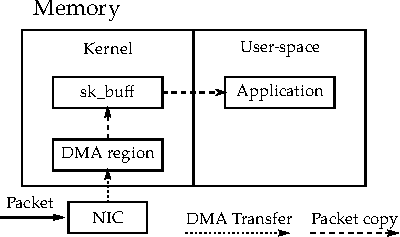
\includegraphics{figures/c05/NAPI}
        \caption{Without PACKET\_MMAP feature}
        \label{fig:NAPI_no_MMAP}
    \end{subfigure}%
    \begin{subfigure}[t]{0.5\textwidth}
        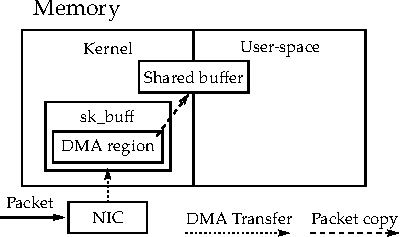
\includegraphics{figures/c05/NAPI_MMAP}
        \caption{With PACKET\_MMAP feature}
        \label{fig:NAPI_MMAP}
    \end{subfigure}
    \caption{Packet transition through memory in Linux NAPI.}
    \label{fig:NAPI}
\end{figure}

The Linux network stack cannot be used for packet capture because the stack takes care of all layers of the packets and delivers only the application content to the application. However, there is an option to use raw packets where the application receives and sends complete packets with all headers, including the Ethernet. The reception of raw packets uses the \emph{sk\_buff} structure and two copy operations are needed for each packet as well. Despite that, the absence of network stack processing provides a large performance benefit. Moreover, it is possible to utilize the RSS feature provided by some NICs and receive packets in different receive queues, which helps to increase performance as well. However, the standard API for working with packets requires performing a system call for reception of each packet (two calls when a timestamp is needed as well), which causes frequent switches between user- and kernel-space.

To provide an efficient way to perform packet capture using standard Linux kernel and drivers, \emph{PACKET\_MMAP}~\cite{LinuxKernelOrganization-2017-PACKETMMAP} feature was added to the kernel. It utilizes a shared buffer between the kernel and the user-space, as shown in Figure~\ref{fig:NAPI_MMAP}. Therefore, the number of packets that can be read in a single batch is not limited, which significantly lowers the number of necessary system calls and thus improves performance. Another advantage of the PACKET\_MMAP feature is that the processing of packets can be performed by multiple threads. The distribution of packets can be performed using a hash, round robin, random selection, and several other policies. 

Although the Linux NAPI has evolved to support fast packet handling, there are several important performance limitations left:
\begin{itemize}
  \item The packets are copied from DMA memory region to the user-space accessible buffers.
  \item The packets are always processed by kernel network stack.
  \item There is little support for NUMA architecture awareness.
\end{itemize}

There are several frameworks that aim to remove these limitations to achieve the highest possible throughput for packet I/O operations.


\subsection{High-Speed Packet I/O Frameworks}

Although there were several works analysing the performance packet capture applications, such as~\cite{Degioanni-2003-Profiling}, one of the first alternatives to using the Linux network stack for packet capture was \emph{PF\_RING}. The PF\_RING socket was created by \citeauthor{Deri-2004-Improving} and its first description appeared in~\cite{Deri-2004-Improving}. The PACKET\_MMAP was very new at that time and some of the introduced features, such as memory mapping overlapped. However, the PF\_RING had several advantages. Firstly, the packets were not queued into kernel network structures at all. It meant, that they were not available to standard applications using socket API but only to applications that used the PF\_RING sockets. Secondly, packet sampling was implemented at a lower level, which meant that sampled packets were not even passed to upper layers. Lastly, multiple applications were able to simultaneously open several PF\_RING sockets without interference. However, the main performance limitations remained the same as with Linux NAPI.

The problem with unnecessary copying between DMA-able memory and the shared buffer was already solved when a specialized NICs with custom drivers were used. One of the most used cards for this purpose was the DAG NIC~\cite{UniversityWaikato--Dag} which was eventually commercialized by the Endace~\cite{ETL--Endace} company. The DAG NIC used FPGA chip that could be programmed to provide specific functionality, such as high-precision packet timestamping. Moreover, it meant that it was possible for the driver to instruct the card to upload packets in a correct format directly to the buffer that was shared to the user-space. \citeauthor{Degioanni-2004-Introducing} used this approach and proposed a design for distributing packets to multiple threads to better utilize CPU parallelism~\cite{Degioanni-2004-Introducing}. However, the card did not support RSS and thus the single buffer to which the NIC uploaded the packets remained to be a bottleneck.

To eliminate unnecessary packet copying even without the use of a specialized NIC, \citeauthor{Deri-2005-nCap} developed a new framework called nCap in \citeyear{Deri-2005-nCap}. The most important innovation was that the standard kernel packet processing was completely bypassed. A specialized driver was developed for compatible NICs (Intel 1\,GE and 10\,GE adapters were supported) that allowed the NIC to directly manage the packet reception and transmission buffers. These buffers were then mapped directly to user-space and a user-space library called nCap is used to manage these buffers. This \emph{zero copy} approach, shown in Figure~\ref{fig:zero_copy}, is used in almost all other high-speed packet frameworks as well. The main disadvantage is that it requires specialized or at least modified drivers and a supported NIC. The direct access to packet buffers filled by the NIC was eventually combined with PF\_RING into the PF\_RING DNA~\cite{ntop-2010-PFRING} (Direct Memory Access) framework. The disadvantage of this approach is that only one application at a time can access the packet buffer.

\begin{figure}[!tb]
  \begin{center}
    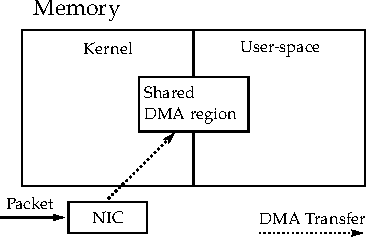
\includegraphics{figures/c05/zero_copy}
  \end{center}
  \caption{Packet transition through memory using a zero copy approach.}
  \label{fig:zero_copy}
\end{figure}

When commodity NICs started to support Receive Side Scaling (RSS), the packet capture frameworks started supporting this feature to better utilize multi-core CPUs. \citeauthor{Fusco-2010-High} showed how RSS can be utilized by multi-threaded polling together the zero copy approach~\cite{Fusco-2010-High} in~\citeyear{Fusco-2010-High}. The basic idea was to use one kernel polling thread for each receive (RX) queue and make the associated buffer available to one user-space capture thread. This approach, called \emph{TNAPI}, was used together with the PF\_RING framework and utilized a custom driver for zero copy packet reception. The authors show that it is important to correctly configure the system to work on NUMA architecture by setting CPU affinity of the individual polling and packet capture threads. Therefore, this approach mitigates the limitations of Linux NAPI discussed in the previous section. 

The development of PF\_RING, nCap, DMA, and TNAPI frameworks resulted in the creation of the \emph{PF\_RING ZC (Zero Copy)} framework~\cite{ntop--PFRING}. It uses proprietary drivers to deliver packets to PF\_RING using the zero copy approach, supports RSS and NUMA architecture to spread packet processing across multiple CPU cores and threads, and allows the kernel networking stack to process packets when no PF\_RING aware application is running. Moreover, by managing the PF\_RING in the kernel, it supports packet fanout for multiple user-space applications and even virtual machines. The PF\_RING ZC also allows user-space applications to receive packets in bursts (batches), which was not possible in vanilla PF\_RING. This feature allows to reduce the number of system calls and significantly helps to increase performance, especially when mitigations to Meltdown and Spectre attacks made syscalls more expensive~\cite{Gregg-2018-KPTIKAISER}.

\emph{PFQ} and \emph{netmap} packet capture frameworks were published 2012. Around the same time, Intel started public development of the \emph{Data Plane Development Kit}. The \emph{PFQ} packet capturing engine was introduced by \citeauthor{Bonelli-2012-Multi} in~\cite{Bonelli-2012-Multi}. PFQ supports RSS, both vanilla and modified drivers (for zero copy operation), and utilizes packet processing within NAPI context. The transition of packets from kernel-space to user-space is implemented by a wait-free queue. When packets need to be copied, it is done in batches which increases performance. The authors showed that the performance of PFQ is better than that of vanilla PF\_RING in their setup. PFQ has evolved significantly in the recent years. The authors added many features~\cite{Bonelli-2014-Purely, Bonelli-2016-Network, Bonelli-2017-Enabling}, such as support for in-kernel programmable early processing and user-space parallel processing while preserving normal host system network stack operation.

The \emph{netmap} framework developed by ~\citeauthor{Rizzo-2012-Netmap} is different from PF\_RING and PFQ in a fundamental way. The packets are not stored in continuous buffers but rather in separately allocated buffers of fixed sizes. It allows passing packets between interfaces in a zero-copy manner. Moreover, a user-space application can exchange packets with the NIC and the host networking stack independently. This design is useful for applications such as packet routing and forwarding.

Intel's \emph{Data Plane Development Kit}~\cite{LFP--Data} known simply as \emph{DPDK} is set of libraries and drivers for fast packet processing. After Intel started the project, it's governance came under the Linux Foundation Project, which unites many companies that contribute to the project. Similarly to netmap, it uses discretely allocated packet buffers instead of buffer ring. However, user-space communicates directly with the card to eliminate unnecessary system calls. Therefore, when a driver with DPDK support is loaded, the NIC cannot be used together with the standard kernel networking stack. By utilizing per packet buffers DPDK allows processing packets out of sequence, which is useful for example for a selective packet capture. Matching packets can be retained while others can be quickly discarded. This is not possible with ring buffer approach without packet copying. DPDK does not support interrupts, therefore packets are always polled from the NIC. This is effective to high loads, however, it excessively utilizes the CPU for lower packet rates. DPDK is widely supported and specialized drivers exist for many NICs from different vendors~\cite{LFP--DPDK}. 

There are other packet capture and manipulation frameworks that were not discussed in this section, such as OpenOnload~\cite{Mansley-2008-Getting} from Solarflare and PacketShader I/O~\cite{Han-2010-PacketShader} using GPU acceleration to build fast router. Moreover, manufacturers of (FPGA-based) high-speed NICs such as Endace, Napatech, Myricom, Mellanox Technologies, or Netcope Technologies provide their own drivers and libraries for fast packet processing together with their products. These drivers and libraries utilize very similar if not the same approaches as the ones described in this section.

There are several works comparing the performance of different packet capture frameworks. They can be used as a reference when choosing the correct framework for a certain use case. \citeauthor{Braun-2010-Comparing} evaluate the performance of native FreeBSD and Linux packet capture together with PF\_RING on Linux~\cite{Braun-2010-Comparing}. They identify bottlenecks and provide guidelines for debugging loss of performance. The authors of~\cite{Garcia-Dorado-2013-High} not only compare the performance of PacketShader, PFQ, and PF\_RING, but they also provide a detailed description of these frameworks and of Linux NAPI as well. \citeauthor{Wang-2016-Comparison} compare PF\_RING, PF\_RING ZC, and DPDK frameworks in~\cite{Wang-2016-Comparison}. The focus of this comparison is on the correct utilization of the NUMA architecture. The authors conclude that the difference in thread assignment between the compared frameworks has an impact on the overall performance. However, they fail to realize that processing on one of the NUMA nodes must be naturally faster since the NIC is directly connected only to this one node. The authors of~\cite{Barbette-2015-Fast} not only compare features and performance of PACKET\_MMAP, PacketShader I/O, netmap, PF\_RING ZC, and DPDK, they also analyse the use of these frameworks with modular router Click. The extensively discuss the impact of important features such as I/O batching, ring size, execution model, zero-copy, and multi-queuing on the final performance of the Click router. Finally, \citeauthor{Gallenmueller-2015-Comparison} propose a model to estimate and assess the performance of various packet processing frameworks in~\cite{Gallenmueller-2015-Comparison}. They apply the model to DPDK, netmap, and PF\_RING ZC. They assess the transmission efficiency, the influence of caches, the influence of batch sizes, and latency for each framework.

% TODO framework comparison table: take from \cite{Barbette-2015-Fast} and add PFQ?


\section{High-Speed Flow Monitoring}

Packet capture is only the first part of the flow monitoring process. After the packet is received by the flow exporter software, it needs to be processed as quickly and efficiently as possible. Packet processing, flow creation, and flow export have been described in Chapter~\ref{chap:network-flow-monitoring} and this section aims to provide an overview of techniques that can be used to accelerate these elements of the flow monitoring process. 

We start with a description of techniques that rely on hardware acceleration which uses special features of the NIC. These features include receive side scaling discussed in the previous section and packet preprocessing. Software acceleration techniques are available regardless of the used NIC and involve effective processing on multiple cores and flow creation design. The Table~\ref{tab:flow-acc-techniques} provides an overview of the discussed techniques. The highlighted techniques are novel and represent our contribution to the high-speed flow monitoring field. We deliberately avoid the use of sampling since it degrades the quality of exported data, as shown by the authors of~\cite{Brauckhoff-2006-Impact}.

\begin{table}[ht!]
    \centering
    \begin{tabular}{l|l}
    \toprule
    \textbf{Hardware acceleration} & \textbf{Software acceleration} \\ \hline
    Receive Side Scaling & Multithreading \\
    Packet trimming & NUMA awareness \\
    \emph{Packet header preprocessing} & \emph{Flow state in parsers} \\
    Flow processing offloading & Flow cache design \\
    \emph{Application identification} & Per-flow expiration timeout \\ 
    & Delayed packet processing \\ 
    & Bidirectional flow records \\ \bottomrule
    \end{tabular}
    \caption{Flow Acceleration Techniques (\emph{Novel Proposals Are Highlighted}).}
    \label{tab:flow-acc-techniques}
\end{table}

This section provides an overview of the flow monitoring acceleration techniques, however, we do not have explicit data to show the direct impact of the presented techniques on the flow monitoring performance. A case study utilizing several of the presented techniques is presented in Section~\ref{sec:performance-high-density} instead. This study shows that it is possible to achieve more than 100 Gb/s throughput on a commodity CPU when hardware-accelerated NICs are used and several acceleration techniques are applied.


\subsection{Hardware Acceleration in Flow Monitoring}\label{sec:performance-hw-acceleration}

Hardware accelerated flow monitoring is based on offloading of parts of the packet or flow processing to the specialized hardware, mainly the NIC. The extent of the offloaded work depends on the capabilities of the NIC. A field-programmable gate array (FPGA) is usually used in hardware-accelerated network interface cards. It allows to parse packet headers and perform tasks such as packet trimming, computing hashes to identify flows or assign timestamps directly in the NICs. It usually supports transferring data to multiple buffers in RAM so that the software can efficiently use a zero copy multi-threading model. As described in the previous section, there are several manufacturers that provide these cards. However, NICs can support hardware acceleration even without an FPGA chip. The capabilities are usually more limited and cannot be extended after the card is produced. For example, Intel produces many NICs, such as the Intel XL710~\cite{IntelCorporation-2014-xl710},  without an FPGA chip that provide basic hardware acceleration such as packet hashing or even timestamping. Use of commodity cards with advanced features like timestamping or packet filtering has been proposed by \citeauthor{Deri-2013-10} in~\cite{Deri-2013-10} in \citeyear{Deri-2013-10}.

We are not the first ones to propose the use of hardware acceleration in flow monitoring. \citeauthor{Antichi-2012-Enabling} proposed to use NetFPGA platform for passive network measurement in~\cite{Antichi-2012-Enabling}. They note that without hardware support, the packet timestamps have poor accuracy. The use of FPGA allows to timestamp, filter or trim the packets, which saves CPU processing time and allows to achieve higher packet rates. However, their work is targeted only on 1\,G environment.

\subsubsection{Receive Side Scaling}
Receive Side Scaling has support in almost all modern NICs. It is used by Linux NAPI to store the received packets to different queues in order to utilize multiple threads for packet processing. The NAPI ensures that packets belonging to a single application always arrive in the correct order even if received by different queues. However, the packet capture frameworks do not usually provide such a guaranty.

Figure~\ref{fig:rss} shows the principle of the RSS. Each packet is processed and a receive (RX) queue is selected. Multiple It allows multiple threads process packets from different queues without any synchronization, therefore the choice of the distribution function crucial. Many applications, including flow processing, require that all packets of the same flow are processed by the same thread. Therefore, the distribution function must put the packets of the same flow to the same RX queue. To achieve this, the distribution function is usually implemented as a hash function that computes a hash from certain header fields of each packet. Note that in case of flow monitoring, these fields must be a subset of flow key, otherwise the flow could be inadvertently split into several RX queues. 

\begin{figure}[t!]
  \begin{center}
    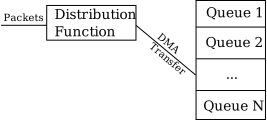
\includegraphics{figures/c05/rss}
  \end{center}
  \caption{Receive Side Scaling Packet Distribution.}
  \label{fig:rss}
\end{figure}

IP addresses and transport layer ports are often used to compute a hash. However, it is often forgotten that fragmented packets do not always have transport layer information present, which can result in fragmented packets being sent to different queue than the rest of the flow. Therefore, it is better, in most scenarios, to use only IP addresses to distribute the flows to different queues.

Often the application needs to process both direction of a communication, e.g. biflow. In such a case, the used hash function must return the same value for both directions. We have proposed to simply order the bidirectional fields (IP address and ports) by value before applying the hash function. This solution is implemented in the HANIC design~\cite{Liberouter--Hanic} of COMBO cards family. Intel NICs allow setting of different RSS hash keys to achieve different hash distribution. Although there are several symmetric RSS hash keys that create the same hash for both directions of the communication, the hash distribution is compromised~\cite{Woo-2012-Scalable}. Therefore, if the hash is used to identify the flow afterward, there are many collisions. We found in our experiments that it is more effective to recompute the hash in software in these cases.

A problem that is often encountered when using RSS is that each NIC supports only a specific set of link layer protocols. When an unknown protocol is encountered, all packets that cannot be parsed are sent to a default queue. Therefore, RSS cannot be effectively used for these protocols. FPGA-based cards can be updated with new firmware, however, commodity cards with a fixed set of features should be carefully chosen when an uncommon link layer protocol is used.

The performance improvement achieved when using multiple queues is directly related to the number of queues and the number of available CPU cores. Since most queues are going to be actively polled under high load, using more queues than CPU cores available is not advisable, as it causes the threads to be switched. However, too many queues also induce a high load on a memory controller causing the performance to be degraded. It is best to experiment with different numbers of queues to find an optimal value for the target system. We have achieved the best results with 8-16 queues, depending on the specific scenario and the number of CPU cores.

\subsubsection{Packet Trimming}

A simple way to lower the memory controller load is to trim the received packets when packet payloads are not required, e.g. for basic flow monitoring. Capturing the first 100 bytes of each packet is usually enough to contain various MPLS, VLAN, Ethernet, IPv6, and TCP headers. The rest of the packet can be discarded. A similar technique can be used when copying packets from kernel to user-space as shown in~\cite{Deri-2004-Improving}. The author uses libpcap with snaplen 128\,B which speeds up packet capture.

However, much better acceleration is achieved when the packets are trimmed by the NIC and only the shortened packets are copied to the RX queues. Although the per-packet processing costs are usually not decreased, this technique significantly helps the memory controller by lowering the data throughput. 

The performance improvement achieved by this method depends on the average length of processed packets. For example, the shortest packets cannot be trimmed at all, therefore packet trimming would not help in some artificial benchmarks. Moreover, application flow measurement requires also the packet payload. The amount of data that can be discarded varies depending on the measured application protocols. Unless the NIC has additional knowledge about measured traffic, it should not trim the packets at all for application flow measurement.

\subsubsection{Packet Header Preprocessing}

Basic flow monitoring usually utilizes only a small subset of packet header fields. Therefore, a more radical way to save memory bandwidth and CPU cycles is to let the NIC extract the information required for flow monitoring and send only a special message with this information to the RAM. This allows the packet processing in the flow exporter to be simplified since it only needs to read the data from a well-defined structure. Moreover, it also helps the memory controller by using only the necessary subset of all available data.

This process requires very specialized FPGA-based cards, such as the COMBO family cards from CESNET. We have successfully used the proposed technique method to build a high-density flow monitoring system. The results are presented in Section~\ref{sec:performance-high-density}.

Even better results could be achieved by the close collaboration of the NIC and flow exporter. If the NIC could send the data in the exact format that is used by the flow exporter, it could be used directly without reordering the elements and filling out internal structures of the flow exporter. In any case, this method is not applicable for application flow measurement since application layer parsing is too complex and dynamic to be fully handled in the FPGA.

\subsubsection{Flow Processing Offloading}
We have shown that packet processing can be offloaded to the NIC almost entirely. However, it is possible to go even further and offload the flow creation process to the NIC as well. It was proposed by \citeauthor{Zadnik-2008-Network} in~\cite{Zadnik-2008-Network} to create a flow cache directly in the NIC. However, this approach is not used in practice as it has two main disadvantages. Firstly, the memory requirements of the flow cache exceed the resources available in most NICs even today. Secondly, the flow exporters often support additional on-demand features such as processing application layer information, or extended monitoring of TCP connection features. These features are hard or even impossible to implement in the firmware of the NICs. To phrase it differently, the NICs are not flexible enough to efficiently keep up with changing demands placed on the flow monitoring.


We have established that packet header preprocessing and packet trimming in the NIC are not usable for application flow monitoring. The main reason is that application layer parsing needs to be done in software. However, most packets do not carry application protocol headers. These packets can be processed by NIC and only extracted information transferred to software. Moreover, once the important features each flow are extracted, the rest of the flow creation process usually consists of simply incrementing various counters. Therefore, it is possible to offload this part of the processing to the NIC. Such a solution is proposed in~\cite{Kekely-2016-Software} and is called Software Defined Monitoring (SDM). It is based on offloading of heavy flows to the NIC. The important information from application layer is usually transferred in first $N$ packets, where $N$ can be expected to be lower than 20 in most cases. Therefore, after the software processing encounters the $N^{th}$ packet, it instructs the NIC to process the rest of the flow. Only aggregated information about the flow is sent from NIC to software. The flow cache in the NIC is rather limited in comparison to the amount of RAM available in the software. However, only heavy flows need to be kept in this cache and it can be expired more often to reduce memory requirements. The authors show that 85 percent of traffic is observed in five percent of heavy flows. Therefore, the benefit of SDM has been shown to be an aggregation of 85 percent of packets to flow records in the NIC. This significant acceleration allows application flows to be monitored on 100\,Gb/s traffic.

Although the SDM is the most efficient solution for offloading part of the flow processing to the NIC, there are disadvantages as well. Once a flow is offloaded to NIC, software parsers cannot observe further payloads containing subsequent application headers. For example, in the case of the HTTP protocol, the HTTP pipelining cannot be detected and information about further requests and responses in the same connection is lost. Therefore, SDM cannot offload flows that are expected to have important data in the payload of future packets. Another problem can occur when an offloaded flow record is expired by the flow exporter, e.g. due to collision in the flow cache. In this case, the NIC is instructed to start sending full packets for this flow again. However, there is a delay in this process and some preprocessed packets might already have been sent to an RX queue. Without an existing flow record, partial information from the preprocessed packets cannot be used to create a new flow record. The reason is that it might be missing some of the link layer information, which is considered to be constant for each flow an thus does not need to be updated with each packet.

\subsubsection{Application Identification}

Packet classification in FPGA is not a novel idea in itself~\cite{Song-2005-Efficient}, however, it was not yet used together with high-speed application flow monitoring. Since only a small portion of all packets carry application protocol information necessary for flow monitoring, it is beneficial to recognize such packets in the NIC and mark them for further processing in the software. As the NIC cannot do complex application header processing, only a simple mechanism, such as pattern matching, can be utilized for packet classification. The work of the WAND Research Group~\cite{Alcock-2012-libprotoident} shows that it is possible to achieve reasonable traffic classification accuracy using only the beginning of a packet payload. 

Once the packets carrying application protocol headers are marked, the software parsers can process only these important packets. Moreover, other packets can be trimmed or parsed in the NIC and only important information can be passed for processing in the software. Packet classification can also benefit the SDM. When a flow is offloaded to NIC and a packet with application protocol header is matched, the preprocessing of such a flow can be terminated and full packets returned to the software. This approach would effectively solve the above-mentioned problem of HTTP pipelining. 

The accuracy and usability of pattern matching for packet classification depend on target application protocols and resource limitation of the NIC as well. Further research is needed to determine whether this method can be used for real-world application flow monitoring.


\subsection{Flow Exporter Software Optimization}\label{sec:performance-sw-optimization}

The performance of flow monitoring can be greatly enhanced by offloading as much of the necessary packet processing as possible to the NIC. However, to build a high-performance flow monitoring solution the software processing must be carefully tuned as well. Moreover, the FPGA-based NICs are much more expensive than commodity NICs and cannot always be deployed. Therefore, we focus on flow monitoring optimizations that can be achieved by careful software design and system configuration in this section.

\subsubsection{Multithreading}

The development of modern CPUs has a tendency to substitute raw power (frequency) for a higher number of CPU cores. To fully utilize the potential of a multi-core CPUs and achieve high flow monitoring performance, it is necessary to create a multithreaded flow monitoring software.

The three main parts of flow monitoring process can be naturally executed in different threads. The first thread receives packets and parses the packet headers. The parsed data are passed to the flow creation thread that manages the flow cache. When a flow is exported from the flow cache, it is passed to the third thread that manages flow export. Figure~\ref{fig:exporter-thread-noRSS} illustrates this execution model, which uses $3$ threads in total.

\begin{figure}[t!]
  \begin{center}
    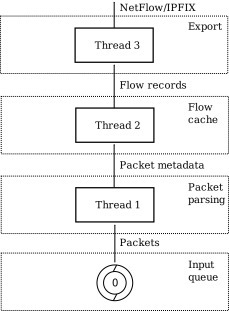
\includegraphics{figures/c05/exporter-thread-noRSS}
  \end{center}
  \caption{Multithreaded Flow Monitoring on a Single Input Queue.}
  \label{fig:exporter-thread-noRSS}
\end{figure}


For NICs with RSS support, the flow processing can utilize more than a single queue. The easiest approach is to have different threads process packets from different buffers. The resulting flow records are aggregated either in a single flow cache or in multiple flow caches, one per each thread, as shown in Figure~\ref{fig:exporter-thread-schema}. In either case, it must be ensured that there is a single thread used for exporting the resulting flow records where the data from multiple processing threads are merged. The latter approach is more effective as it clearly prevents the flow cache to become a point of contention. However, when there are multiple flow caches, it is necessary to ensure that each flow is aggregated in a single flow cache as previously described in the passage about Receive Side Scaling. Using this approach, $N+2$ threads in case the first case or $2N+1$ threads in the second case can be utilized, where $N$ is the number of buffers. The last thread is used for flow export. 

\begin{figure}[t!]
  \begin{center}
    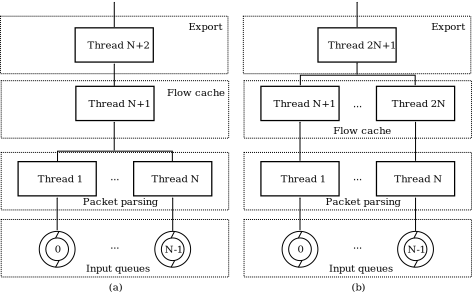
\includegraphics{figures/c05/exporter-thread-schema}
  \end{center}
  \caption{Multithreaded Flow Measurement with a RSS Support: a) Single Flow Cache; b) Multiple Flow Caches.}
  \label{fig:exporter-thread-schema}
\end{figure}

Using $2N+1$ threads for flow processing results in $17$ threads for $8$ RX queues. On a system with lower number of cores, it is desirable to use fewer threads so that each active thread has a dedicated core for itself. This helps to avoid the necessity to execute different processes and threads on the dedicated cores, which increases performance. Moreover, having the same data to be processed by multiple threads increases the impact on the memory controller, which can become overloaded for a large number of threads. Therefore, lowering the number of cores per RX queue can, in fact, help the performance. By combining packet processing and flow cache to a single thread, the total number of threads can be lowered to just $N+1$ while retaining multiple flow caches. Whether to combine the threads or not depends on the throughput of the memory controller, CPU frequency, number of cores and the actual amount of work performed by each thread. The measurement framework proposed by the authors of~\cite{Gallenmueller-2015-Comparison} can be used to determine the characteristics of the system.

% TODO pridat obrazek se N+1 thready pro spojeny packet processing a flow cache?

Another reason to keep packet parsing and flow cache in a single thread is that the packet parsing and processing of application protocols may require a state of the connection to be kept. In such a case the flow cache record must be made available to the packet processing thread. If the threads were to be kept separate, it would result in a use of synchronization primitives and overall performance decrease. One possible solution to this problem is to keep a different, smaller cache for chosen flow records directly in the packet processing thread. However, it is much more simple to use the flow cache directly when the packet parsing and flow cache are managed in a single thread.

\subsubsection{NUMA Awareness}

To build a high-speed flow monitoring system, servers with multiple CPUs are often used. However, special care must be taken to deploy such a configuration properly. Modern systems use Non-Uniform Memory Access (NUMA) architecture where each CPU has direct access to single \emph{local} memory bus and a high-speed interconnect (such as QPI) must be used for communication between different nodes (CPU reading from a \emph{remote}, without a direct access). Moreover, each NIC is directly connected to only one CPU. Therefore, allocating DMA buffers for the packet reception in a remote memory is ineffective as it needs to use the high-speed interconnect between the CPUs.

The generic rule is to avoid using remote memory as much as possible. Therefore, the buffers for the RX queue should be allocated on the CPU connected to the NIC. However, when multiple CPUs are used for processing packets, it makes sense to distribute the buffers to those CPUs. The threads processing packets should always run on a local core, which can be achieved by setting the affinity of the thread to the CPU of the specific core. When starting new core, it is important to first set its affinity and only then allocate memory as the memory is allocated on the local core by default. If the thread is migrated to a different CPU, the local memory becomes remote.

If biflow creation is not required, it is possible to utilize two NICs to process different directions of the traffic. Each can be connected to different CPU, which eliminates the need to share data between CPUs almost entirely.

\subsubsection{Flow State in Parsers}

It is not effective to try every available application header parser on every packet to see which one is able to process it. When a packet from a flow was already matched by some application parser, it will usually not be matched by others. Therefore, by keeping the information about which flow is to be processed by each parser, most of the unnecessary and possibly expensive calls to application parsers can be eliminated. Moreover, when the flow is yet unmatched by any application parser, it is best to execute the application protocol parsers from the most common to the least common protocol.

Moreover, when the flow state is known to the parser, an optimization similar to the SDM can be deployed. When an application parser detects that it has already obtained all important information from a given flow, it can instruct the exporter to skip processing of the application layer for this flow. This way the different application parsers can opt-out from processing individual flows.

This optimization can be applied especially to the encrypted traffic using SSL/TLS protocol. It is quite easy to detect TLS encryption from the specific format of its handshakes. Without the means to decipher the traffic, other application parsers cannot process encrypted packets. Therefore, all other applications parsers can be skipped when the SSL/TLS protocol is detected. Since HTTPS adoption is steadily increasing~\cite{Felt-2017-Measuring}, the amount of SSL/TLS connections rise as well, therefore this optimization is likely to gain impact in the future.

\subsubsection{Flow Cache Design}

One of the most performance critical parts of any flow measurement software is the flow cache. The cache needs to be designed to hold hundreds of thousands of flow records, do fast inserts, lookups, updates, and manage record expiration after active and inactive timeouts. It also needs to be robust and resilient enough to handle excessive workloads during DDoS attacks~\cite{Sadre-2012-Effects}. 

The flow cache design has been studied in the literature, for example, in~\cite{Wang-2011-Memory, Nassopulos-2014-Flow}. Although authors propose to use various data structures such as linked lists, trees, or multidimensional hashing table, our experience using a hash table indicates that the simplest structure provides the best performance. The flow cache has to maintain data locality to make good use of CPU caches, therefore the dynamic structures do not perform as well as the simple hash table. To avoid collisions, the flow record can be placed in any of the $N$ positions after the computed one. Therefore, the record is always found in constant time and no overflow structures are necessary. However, the flow cache utilization never effectively reaches 100 percent as that would cause too many collisions. It is best to estimate the maximum number of flow records that needs to be kept at a time and choose the cache size so that there are no or only little collisions for this number of records. Each collision necessitates a forceful export of a flow record, which leads to performance degradation.

Implementation of active timeouts is straightforward. Each time a packet is being added to a flow record, the start time of the flow record is compared to the packet timestamp. When the difference is greater than active timeout, the flow record is exported and a new flow record is created in its stead. However, inactive timeouts are more complex to implement effectively. Different algorithms using time-ordered linked lists and last least recently used structures were proposed in the literature. However, management of such structures is costly. A straightforward approach would be to start an auxiliary thread that would search the cache for any flow records that need to be expired. However, this would cause heavy locking on the flow cache, which is undesirable as well. The the most efficient way to implement inactive timeouts on a hash table flow cache is to have the thread managing the flow cache check several records each time a packet is received. This approach avoids locking the flow cache and performs well. However, the export of inactive flow records may be slightly delayed. Moreover, the search for expired flows must be performed even when no new packets are received. Carefully balancing the flow cache management tasks is a complex problem which offers a considerable potential for further research.

The length of flow records that are kept in the cache has an impact not only on the size of the flow cache but on the performance as well. Having too long flow records causes more cache misses during while working with the cache. For example, when an URL is extracted from an HTTP application header, it can be thousands of bytes long. Reserving place for this kind of information in the flow record is impractical and hurts performance. Our measurements show that it is faster to dynamically allocate memory for application data of certain size and store only a pointer in the flow record itself. The less common the application is, the more beneficial is to allocate the space for its data dynamically since only a small amount of these allocations is performed in comparison to every flow record being significantly larger.

\subsubsection{Per-Flow Expiration Timeout}

Flow cache inactive timeout expiration has a large impact on the performance, as discussed in~\cite{Rodriguez-2013-Empirical, Molina-2006-Design}. However, the value for the timeout is usually the same for all flow. The authors of~\cite{Rodriguez-2013-Empirical} show that different classes of traffic could use a different inactive timeout. To implement this in application flow monitoring, we propose that the timeouts should be configurable per flow. When a flow is successfully processed by an application parser, a timeout appropriate for this application should be assigned. This approach should decrease the memory requirements and increase overall performance of the flow monitoring.

Flows that comprise only of a single packet represent a special traffic class. If the flow exporter is able to detect and decide that the first packet is also the last one, the flow can be directly exported and does not need to enter the flow cache at all. This is especially useful to cope with DDoS attacks, as described by~\citeauthor{Sadre-2012-Effects} in~\cite{Sadre-2012-Effects}. Moreover, it could be used for monitoring of DNS traffic as well since most of the request and responses consist of only a single packet.

\subsubsection{Delayed Packet Parsing}

Processing application layer is often a complex task that needs to be performed in the most performance sensitive situation, during packet parsing. However, the extracted information is often just stored in the flow record and is not used in the flow monitoring process itself. We have already discussed that in some cases it is preferable to allocate memory for application data dynamically. We can take this concept further and extract only the necessary information during packet parsing (e.g. HTTP method) and store the pointer to the copy of the rest of the application data from the packet. The rest of the data can be processed in a less critical section of the flow monitoring process, such as in the flow export thread. 

The delayed packet parsing improves performance especially in cases when the application data are too large to be kept directly in a flow record and memory allocation is performed in any case. As always, the impact of this optimization needs to be carefully examined as it depends on the utilization of individual threads and composition of the monitored traffic.

\subsubsection{Bidirectional Flow Records}

Biflow processing can improve performance. The reason is that the shared data (IP addresses, protocol, and ports) are stored only one, which reduces memory footprint. Moreover, since both sides are often communicating at the same time, there is an improved chance that the bidirectional flow record will be still cached by the CPU. Even when uniflow is required by the flow data processing software, the biflow can be used and then converted to uniflow during the flow export process.


There are many other optimizations that can be performed to increase application flow monitoring performance, such as efficient flow key computation, packet processing in batches, ensuring CPU cache line alignment of flow records and so on. However, they are mostly a code micro-optimization no different from fine-tuning any other high-performance application and are out of the scope of this thesis.


\section{High-Density Flow Monitoring}\label{sec:performance-high-density}

A current commodity hardware for high-speed network traffic flow monitoring usually consists of a PC with one or two network interface cards (NICs) with a 10\,G Ethernet interface. The role of the hardware is merely to capture the data from the network. The hardware setup is supplemented by open- or closed-source software performing the subsequent steps of the flow monitoring process.

While one can deploy multiple such probes for monitoring of multiple lines, it may not be the best option because of an increased power consumption, a large rack space footprint and a general complexity of the monitoring system management. Our work therefore focuses on exploring the scalability of this concept in a single PC from the performance point of view. There are obviously concerns about various possible bottlenecks of a single PC setup. To name a few: throughput of the NIC, system bus (i.e. PCI Express) and PC memory subsystem, performance of a single CPU core, overhead of potential inter-core or inter-CPU communication.

By using custom-built NICs, we are able to perform experiments with the speeds beyond what is available in the commodity hardware market. The programmability of our FPGA-based NICs allows us to examine the effect of various additional hardware features, such as a packet header preprocessing or a packet trimming. We suggest that some of these features should be included in the next generation of commodity NICs to aid the performance of future network traffic monitoring systems.

The aim of our work described in this section is to identify bottlenecks and potentials for new features of current and near-future monitoring systems, as well as to demonstrate limitations of current CPUs and generally the PC architecture in the particular use case of network flow monitoring. We test a monitoring setup that can be achieved using commodity NICs, then we present impacts of the features provided by our NIC. Last but not least, we compare two different CPUs in the same conditions to determine the influence of CPU choice on the monitoring performance.

This section is structured as follows: Subsection \ref{subsec:high-density-monitoring-architecture} describes our monitoring architecture and how it is different from current commodity NICs. Subsection \ref{subsec:high-density-methodology} explains our experiments and methodology, while Subsection \ref{subsec:high-density-results} presents the obtained results. The last Subsection \ref{subsec:high-density-conclusions} draws conclusions from the results.

\subsection{Monitoring Architecture} \label{subsec:high-density-monitoring-architecture}

This subsection describes our monitoring setup from hardware to software. We briefly introduce our custom-built FPGA-based NIC architecture. We utilize these NICs to incorporate multiple 10\,G interfaces in one box.

\subsubsection{Hardware}

We use the COMBO-80G card~\cite{Liberouter--COMBO} to receive the network traffic. The card is equipped with two QSFP+ cages, which can be set to 4$\times$10\,G Ethernet mode each, thus creating eight 10\,G interfaces in total. The packets undergo a configurable processing in the FPGA and are sent to the host RAM via the PCI-Express gen3 x8 bus. Theoretical throughput of this bus is 64\,Gbps, but due to the protocol overhead, the real-world throughput is slightly higher than 50\,Gbps. Figure \ref{fig:hw} shows the functional scheme of the described hardware.

The FPGA firmware of COMBO-80G has several features that set it apart from conventional NICs and help to improve general throughput when receiving packets. The card automatically assigns a 64-bit timestamp to each packet at the moment of reception. The timestamp has a resolution of one nanosecond, which is better than what can be achieved by assigning it later by the software application. Also the processor load associated with the timestamp generation is removed.

Another feature is a configurable packet trimming. The card can be set to trim the packets to a predefined length, thus saving the PCI Express and memory subsystem bandwidth, most notably for long packets. This feature is clearly intended for the purpose of flow monitoring, since the relevant information (packet header) is at the beginning of each packet.

Further extension of this feature leads to packet parsing directly by the card and transferring only the parsed packet header fields to the host RAM. In addition to bandwidth saving, the processor load is also reduced, because it no longer needs to perform the packet parsing operation. The parsed fields are sent in the so-called Unified Header (UH) format which has fixed structure and thus removes the need for complicated parsing conditions in the corresponding processor code.

To better utilize current multicore CPUs, the firmware features an option to distribute the packets into eight independent DMA channels. Target channel number of each packet is computed by hashing several fields of the packet header, such as IP addresses, protocol, port numbers. This ensures that there is a consistent mapping of network flows to the DMA channels, so that the software threads always see complete flows. In common traffic with large number of flows, the traffic is evenly distributed among the DMA channels.

\begin{figure}[t]
    \centering 
    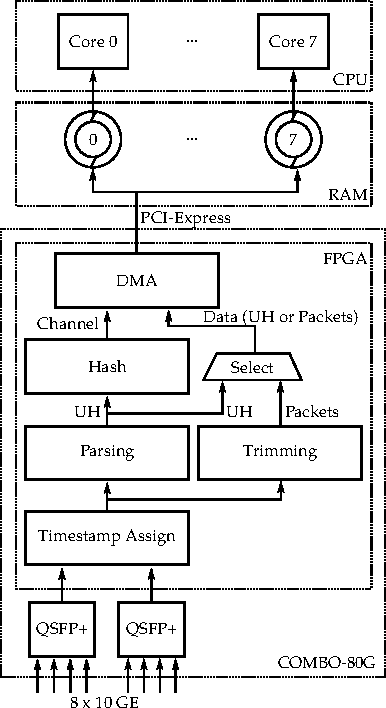
\includegraphics{figures/paper-highdensity/fig/hw}
    \caption{Hardware scheme of single card setup.}
    \label{fig:hw}
\end{figure}

\subsubsection{Software}

The DMA transfers themselves are simplified and optimized to bypass an OS kernel network stack. Large ring buffers are allocated in RAM during the OS driver initialization, and the packets are then uploaded to these buffers by the card almost autonomously. The only communication between the driver and the card is an exchange of buffer start and end pointers (which mark an empty and free space in the buffer), and configurable interrupts generated by the card. The OS driver never touches or even copies the packets, it only maps portions of the buffers to user-space applications. This way the overhead of software processing is minimized and maximum CPU time is left for the application itself. Directly mapping the ring buffers memory to user-space also ensures that the data are copied only once, from the NIC to the RAM. This decreases the load of the memory subsystem, which helps to increase the overall performance.

Data from the ring buffers are processed by a flow exporter. We use FlowMon exporter~\cite{FlowmonNetworks--Flowmon} software which utilizes a multithreaded design to distribute the computational load on multiple CPU cores. The flow exporter architecture is shown in Figure~\ref{fig:exporter}. Input threads read packets from ring buffers and parse L2 to L4 headers to flow records. These flow records are passed to a flow cache which performs flow record aggregation. Expired flow records are exported using single unifying thread, which accepts the flows from all flow caches. Single thread is enough for this task, since is is much less performance demanding.

\begin{figure}[t]
    \centering 
    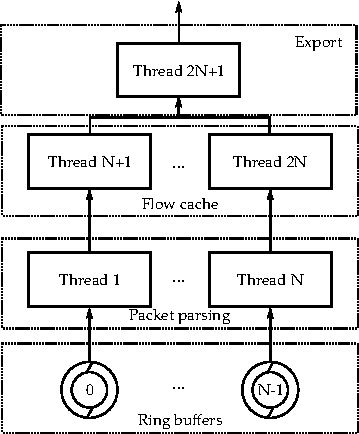
\includegraphics{figures/paper-highdensity/fig/exporter}
    \caption{Flow Exporter Multithreaded Architecture.}
    \label{fig:exporter}
\end{figure}

\subsection{Methodology} \label{subsec:high-density-methodology}

This subsection describes the setup for our experiments. We present our testbed as well as network traffic data that were used to measure the monitoring performance. Successfully processed packets per second and CPU utilization are measured to quantify the performance.

\subsubsection{Testbed Setup}

The testbed consists of two devices. The first is the flow monitoring probe and the second is a packet generator which generates traffic that is measured by the probe.

We use Dell PowerEdge R720 server with two Intel Xeon E5-2670 v1 CPUs as the flow monitoring probe. Each CPU features eight physical cores (16 with hyperthreading), 2.6\,GHz operating frequency (3.0\,GHz to 3.3\,GHz in Turbo mode) and 20\,MB of cache. Maximum TDP of each CPU is 115\,W. The memory controller has throughput of 51.2\,GB/s. Each CPU has four RAM modules available, running at 1600\,MHz with the capacity of 8\,GB per module (64\,GB total). Two COMBO-80G cards are used to receive and process packets. The operating system is standard Scientific Linux release 6.5 running kernel version 2.6.32-431. The whole setup is a 2U standard rack mount PC.

Since the probe has two CPUs, we need to consider NUMA architecture specific setup. Each CPU has a directly accessible portion of RAM, which corresponds to the four physical RAM modules associated with the CPU. Accessing the memory of the other CPU is more costly, since the data need to be passed between the processors using QuickPath Interconnect bus (QPI)~\cite{IntelCorporation-2009-Introduction}. Each PCI-Express bus is also connected to one CPU. This CPU receives the interrupts of connected devices and the devices can write directly to the associated memory using DMA transfers. Therefore, the optimal setup is to have each COMBO-80G card on the PCI Express bus connected to different CPU. The memory allocated by the drivers for the NIC should belong to the same CPU and the flow exporter should also run on this particular CPU. This way, we can almost completely avoid QPI communications when processing the network traffic, which leads to higher performance. However, current version of the NIC drivers does not support NUMA specific memory allocation, which causes inefficient memory access through the QPI bus. The impact of this deficiency is described in Subsection~\ref{subsec:high-density-results}.

We run one instance of flow exporter on each physical CPU. This allows each exporter to use the memory of this CPU for the flow cache and therefore avoid to accessing the flow cache data through QPI.

\subsubsection{Data Generator Setup}

The test traffic is generated by Spirent TestCenter hardware generator at the speed of 10\,Gbps and is replicated to all sixteen input ports. Since the data on all 10\,G ports are the same, we use interface numbers in the flow creation process to ensure that the same packets from multiple interfaces will create different flows. It also ensures that the timestamps seen by flow the exporter are monotonous.

We use an artificial traffic pattern for the flow monitoring performance measurement. This approach has several advantages. Firstly, we can test the worst case scenario using short packets to achieve the highest packet per second ratio. Secondly, it is easy to repeat the tests in another laboratory. Moreover, it is infeasible to simulate a real traffic using packet generators, especially at 10\,Gbps speed. To compensate for different number of concurrent flows and real traffic distribution of packets in flows, we repeat the tests with several different flow counts. All generated data are simple UDP packets, flows are created by permuting parts of IP addresses. The results provided in Subsection~\ref{subsec:high-density-results} are averaged from several measurements taken for each scenario.

Table~\ref{tab:test-data} shows combinations of packet sizes and flow counts used in our measurements. Corresponding packet and bit rates are also shown. Various bit speed is caused by the Ethernet protocol overhead, which is lower for longer packets. All values are given for a single 10\,G packet generator. Since the traffic is repeated to every input interface, the actual flow count and traffic rates sent into our monitoring device are 16 times higher.

The flow count has high impact on the flow cache performance. With the increasing number of active flow records, the memory is accessed more randomly and the CPU experiences more cache misses, which results in higher latency of memory access and therefore in lower performance. It is difficult to estimate the number of flows to simulate from real network, since the real flow records are not updated periodically and the number of active flows in the flow cache at any given moment depends heavily on active and inactive flow cache timeouts and other software settings. Therefore, we test several different options to estimate the influence of flow count on the overall performance. We believe that the highest number of flow count used in our tests is more performance-demanding than real traffic in most networks.

\renewcommand{\arraystretch}{1.1}
\begin{table}[!t]
        \centering
        \begin{tabular}{rrrr}
        \toprule
        \textbf{Packet size} & \textbf{Flow count} & \textbf{Packets/s} & \textbf{Bits/s}\\ \midrule
        64\,B & 128 & 14880545 & 7618839040 \\
        64\,B & 16384 & 14880545 & 7618839040 \\
        64\,B & 131072 & 14880545 & 7618839040 \\ \midrule
        128\,B & 128 & 8445715 & 8648411900 \\
        128\,B & 16384 & 8445715 & 8648411900 \\
        128\,B & 131072 & 8445715 & 8648411900 \\ \midrule
        256\,B & 128 & 4528861 & 9275108100 \\
        256\,B & 16384 & 4528861 & 9275108100 \\
        256\,B & 131072 & 4528861 & 9275108100 \\ \midrule
        512\,B & 128 & 2349560 & 9623786500 \\
        512\,B & 16384 & 2349560 & 9623786500 \\
        512\,B & 131072 & 2349560 & 9623786500 \\
        \bottomrule
        \end{tabular}
        \caption{Combinations of Packet Lengths and Flow Counts Used in the Tests.}
        \label{tab:test-data}
\end{table}


\subsection{Results} \label{subsec:high-density-results}

The results of our experiments are presented in this subsection. We show the measurement performance in a setup achievable by commodity NICs, then we present the improvements achievable by our NICs. Moreover, we show a difference in performance for two different CPUs. We use packets per second as a measure for system performance. Bytes or bits per second can be gained easily by multiplying the number of packets per second by their respective sizes.

\subsubsection{Basic Performance}

First, we have measured the basic performance of the flow exporter on full packets. Figure~\ref{fig:pkt-full} shows packet rates separately for each of the cards. We group the rates for the same packet lengths together. Each group has three pairs of columns. Each color represents a different number of flows per interface. Shades of the color differentiate the NICs. The \emph{Maximum Ethernet} column is the highest achievable aggregated throughput of all 16 Ethernet input interfaces. The \emph{Maximum PCIe} column has been measured by counting the packets received by the simplest possible software application (a packet counter). This way, we get an upper limit on number of packets, that the flow exporter can receive via the system bus.

\begin{figure}[!htb]
    \centering 
    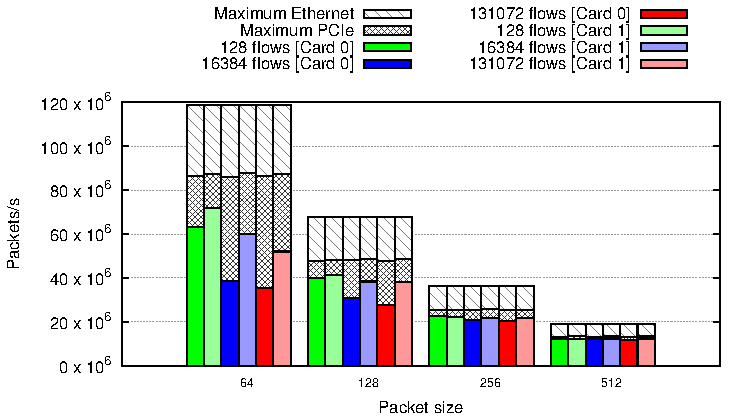
\includegraphics{figures/paper-highdensity/graphs/packets-full-cards.pdf}
    \caption{Full Packet Processing Performance in Packets/s.}
    \label{fig:pkt-full}
\end{figure}


We plot the CPU utilization in Figure~\ref{fig:cpu-full}. The interpretation of the graph is almost the same as for Figure~\ref{fig:pkt-full} with the exception that values for both cards are summed up and the utilization is shown for different flow exporter threads instead. The darker color represents the input thread and the lighter color marks the values for the flow cache thread.

\begin{figure}[!htb]
    \centering 
    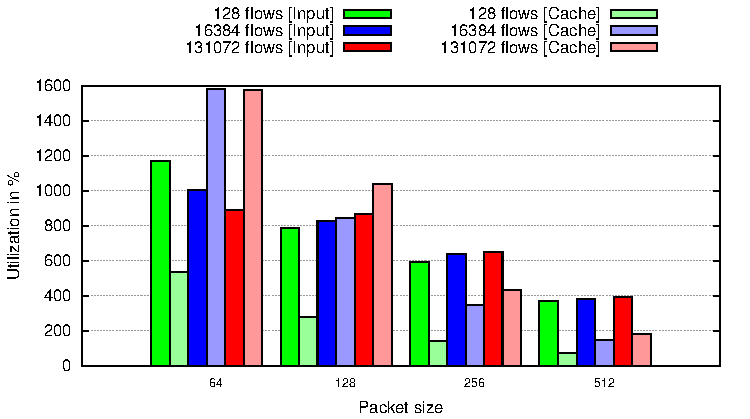
\includegraphics{figures/paper-highdensity/graphs/cpu-full.pdf}
    \caption{Full Packet Processing CPU Utilization.}
    \label{fig:cpu-full}
\end{figure}

There are several important observations that can be made from these two graphs. The performance impact of number of flows is significant, especially for short packet lengths. This is caused by a high number of updates that must be performed in the flow cache. For a smaller number of flows, the CPU can keep a larger portion of the flow records cached in a faster memory. As the number of flows increases, the memory is accessed more at random, which causes more cache misses and eventually a performance decrease. Figure~\ref{fig:cpu-full} clearly shows, that the utilization of the flow cache thread rises with number of flows for all packet lengths.

Performance of the second card is always higher than that of the first card. We attribute this to the device driver, which allocates packet buffers without considering the heterogeneity of the NUMA architecture. In our case, the first card and the corresponding flow exporter always access the RAM through the QPI bus using memory subsystem of the other CPU, which decreases the performance.

Although it seems that the performance is decreasing for longer packets, this depends on the point of view. The number of bytes per second is actually increasing for longer packets. Since less packets need to be processed to achieve the same throughput, the CPU utilization decreases. However, more data are processed, which requires higher memory controller throughput. Therefore, for longer packets, the performance is not hindered by insufficient CPU frequency, but by high memory bus utilization.


\subsubsection{Hardware Accelerated Performance}

Secondly, we have measured the performance using hardware acceleration. Two different acceleration methods have been used. The first method is to set up the COMBO-80G cards to trim the packets to 64 bytes. This allows to keep the processing speed the same for all packet lengths. The second method uses internal parser of the NIC and sends only a predefined data structure, called Unified Header, with parsed information to the software. The main advantage is that the flow exporter does not have to parse the packet headers and therefore saves some CPU time. The disadvantage of both methods is that the flow exporter cannot perform any payload dependent analysis.

Figure~\ref{fig:pkt-all} shows the performance comparison of the processing of full packets, trimmed packets and unified headers. We plot the graphs for 16\,384 flows per interface, but the results are very similar for other flow counts. Note the throughput of PCI Express bus. Using the Unified Headers decreases the number of bytes that must be transferred for each packet. Therefore the throughput is higher even for the shortest packets.

\begin{figure}[!htb]
    \centering 
    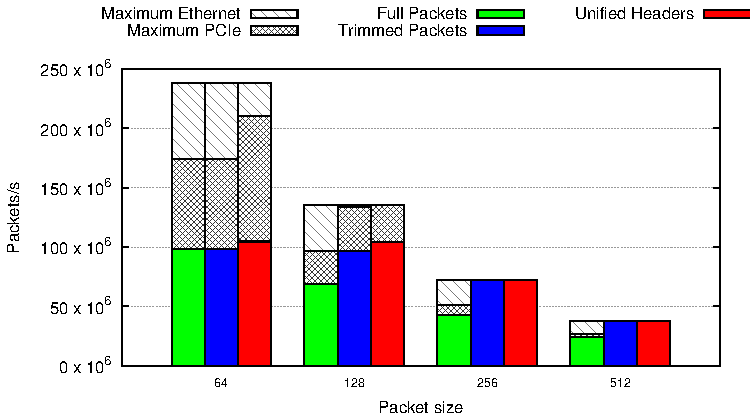
\includegraphics{figures/paper-highdensity/graphs/packets-all.pdf}
    \caption{Packet Processing Performance Comparison in Packets/s for 16\,384 Flows per Interface.}
    \label{fig:pkt-all}
\end{figure}

Using trimmed packets does not achieve any improvements for the shortest packets. However, it allows to transfer almost full Ethernet speed on 128\,B packets to software. Full line rate transfer can be achieved for 256\,B packets using packet trimming or using Unified Headers even for 128\,B packets.

The CPU utilization, shown in Figure~\ref{fig:cpu-all} should be the same for full and trimmed packets for same packet rate. The difference is caused by the fact that higher packet rate can be achieved using trimming. Utilizing the Unified Headers brings the advantage of easier data processing. Therefore, the input thread is always less utilized for the Unified Headers than for trimmed packets. Using the Unified Headers also brings higher performance. The parsing of more complex L3 and L4 headers also causes memory accesses. When it is reduced, more bandwidth is left for the flow cache, which increases the overall performance.

\begin{figure}[!htb]
    \centering 
    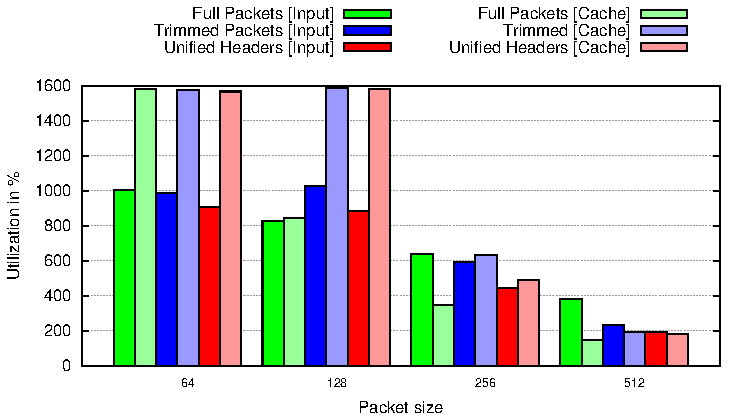
\includegraphics{figures/paper-highdensity/graphs/cpu-all.pdf}
    \caption{Packet Processing Comparison Using CPU Utilization for 16\,384 Flows per Interface.}
    \label{fig:cpu-all}
\end{figure}

\subsubsection{Impact of CPU Choice}

We have also investigated the impact of the choice of CPU on the packet processing performance. We performed the same tests in the same server with different CPUs. We chose E5-2620 v1 CPUs, which represents a cheaper and therefore slower alternative. Each CPU features six physical cores (12 with hyperthreading), 2.0\,GHz operating frequency (2.5\,GHz in Turbo mode) and 15\,MB of cache. Maximum TDP of each unit is 95\,W. The memory controller has throughput of 42.6\,GB/s.

Figure~\ref{fig:packet-trim-comparison} shows a comparison of the performance for the trimmed packets method. The darker colors are used for the faster CPU. The difference is bigger for smaller number of flows and is reduced with growing utilization of the flow cache. On 64\,B packets the performance drop using the slower CPU is 29\,\% for 128 flows, 23\,\% for 16\,384 flows and 21\,\% for 131\,072 flows. 

\begin{figure}[!htb]
    \centering 
    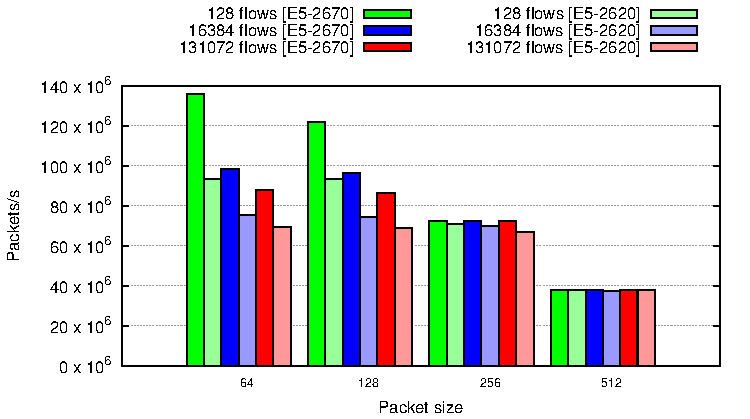
\includegraphics{figures/paper-highdensity/graphs/packets-trim-comparison.pdf}
    \caption{Trimmed Packets Processing Performance Comparison for Two Different CPUs.}
    \label{fig:packet-trim-comparison}
\end{figure}

We assume that the main difference in the performance is caused by the number of CPU cores. Since there are eight independent DMA channels for the data transfer, the best performance is achieved by eight threads processing the data. However, when only six cores are available, the threads must share the cores and the overhead of switching the threads increases. The difference in the frequency helps mostly for parsing the data, therefore it is useful mainly on full packets. Another bottleneck is caused by the memory controller, since the flow cache updates generate lots of random memory accesses. Using a CPU with wider memory bandwidth helps to alleviate this issue.

\subsection{Conclusions} \label{subsec:high-density-conclusions}

The demand for high-density network flow monitoring solutions is increasing. We have built a 2U standard rack server with two COMBO-80G cards. Each card has two 40\,G interfaces and can be used in 8$\times$10\,G mode. Therefore, the server is theoretically capable of monitoring sixteen 10\,G lines, 160\,Gbps in total.

We have used a packet generator to fabricate a traffic of different properties and used this traffic to test the capabilities of the monitoring solution. We have worked with different packet lengths and different numbers of active network flows.

Firstly, we have measured the monitoring throughput on full packets, which is a setup that can be achieved using any commodity card with a timestamping unit and an effective distribution among CPU cores. We have shown that the monitoring performance does not achieve the highest possible rate for short packets. However, the maximum rate allowed by the PCI Express bus is achievable for longer packets.

There are several caveats that need to be kept in mind while working with NUMA architecture. Each NIC is connected to one CPU and should store packets in the memory of that CPU. This needs to be enforced by the driver of the NIC. Consequently, the flow exporter for the NIC should also run on the same CPU and work with the corresponding memory. The drivers that we use are not NUMA-aware and the deficiency is clear from the results.

Secondly, we have shown the impact of hardware acceleration on the the flow measurement. Using a packet trimming ensures that the packet rate that can be achieved for short packets applies for longer packets. This technique allows us to monitor full speed 16$\times$10\,G Ethernet for 256\,B packets. For comparison, the average packet length of our organization's border lines is over 800 bytes. When the packet parsing is performed by the NIC and the information from packet headers are passed using the Unified Headers, the performance is increased even more. The CPU utilization is also lower, since the packet header parsing is a CPU intensive task. However, this approach trades high performance for monitoring flexibility.

The purpose of the last test was to show the difference that can be achieved by using faster CPUs. We have shown that the performance on short packets can rise by more than 30\,\% when using faster CPUs with higher memory bandwidth. We conclude that the monitoring system can achieve even higher performance by utilizing better CPUs. However, a cost to performance ratio is also important for a production use.

More attention needs to be paid to packet loss management. While we aim to achieve a lossless flow monitoring, packets are lost in extreme scenarios nonetheless. In our case, the packets are lost by the NIC at the input when the input buffers are full and DMA transactions are stalling. Therefore, by blocking a single DMA channel packets are lost for all channels. This is clearly suboptimal since the other cores cannot process more packets while their RX queues are not receiving packets as well. An improved design will be implemented in the future where the packets will be dropped before for each DMA channel separately.

There are several improvements that can be made to achieve higher performance. We can buy better CPUs, but the budget for monitoring systems is often limited. The driver for the NICs should be made NUMA-aware to avoid costly memory accesses using QPI bus. Moreover, the current driver allows to read only a single packet at a time. Therefore, processing packets in batches could be used to achieve better performance. We have also shown that features like packet trimming can significantly improve the performance of flow monitoring systems. If the next generation commodity cards should be used for the network flow monitoring, such features can turn out to be crucial for handling large volumes of data. The performance of the PCI Express bus can be doubled by using 16 lanes, which is an approach that can be expected to be used in the future.

\section{Summary}\label{sec:performance-summary}

This chapter has discussed the performance of flow monitoring systems. We have explained different methods of measuring the overall performance and have shown that it is important to choose the one that provides more appropriate results. Different factors that have an impact on the flow monitoring were considered as well. We have shown that the used hardware, system settings, used packet capture framework, settings of the flow exporter, and the used traffic mix have a considerable impact on the results of the measurement. CPU processing power and memory controller throughput are the most obvious bottlenecks for flow monitoring. We have shortly discussed ways to detect these bottlenecks and decide, whether the memory footprint or CPU cycles need to be optimized

The performance of flow monitoring significantly depends on the performance of the underlying packet capture framework. We have presented the evolution of the state-of-the-art packet capture frameworks. Linux NAPI can be used for packet capture on gigabit networks, however, to achieve full packet capture on 10\,Gbps and faster networks, specialized NIC drivers together with kernel network stack bypass must be used. Zero-copy approach and receive side scaling are a necessity to achieve these speeds. The buffers to which the NIC delivers packets through DMA transfers are mapped directly to the user-space. Interrupts are usually disabled at high speeds and extensive polling is performed by the receiving application. When the data needs to be shared between multiple applications, the RX queues are managed by the kernel driver. In this case, the provided API must enable reception of multiple packets at once, a technique called batch or burst packet processing, to avoid unnecessary context switches between kernel and user-space. In case only a single user-space application is processing the packets, such as in case of the DPDK framework, the RX queues are managed directly by user-space, which increases the performance due to the lesser number of context switches.

Although packet capture is an important part of the flow monitoring process, many optimization techniques can be applied to the flow monitoring as well. We have discussed the possibility of hardware acceleration using specialized FPGA-based NICs that allow offloading of part of the flow processing to the NIC itself. We have shown that depending on the capabilities of the NIC, different levels of offloading can be achieved. However, the flow exporter must be aware of these capabilities and actively cooperate with the NIC. Multiple optimizations can be used in the design of the flow exporter software as well. We have argued that multithreading and NUMA awareness are key to flow monitoring performance, although special care needs to be taken to configure the setup correctly. Other optimization techniques such as flow cache design, per-flow expiration timeouts, delayed packet parsing, and the use of biflows have been considered as well.

Finally, we build a high-density flow monitoring system capable of processing 16x10\,Gbps. The system utilized two FPGA-based NICs that allowed us to test the offloading of packet processing. We have shown that this technique allows processing significantly higher amount of traffic. The number of concurrent flows that needed to be kept in a flow cache has had a considerable impact on the measured performance. Moreover, we also demonstrated the importance of having powerful enough CPU by repeating the tests with two different CPUs. We believe that by utilizing more of the proposed optimization techniques, we should be able to achieve even higher throughput of the system, possibly reaching even 200\,Gbps rate offered by the latest NICs available on the market.